\documentclass[14pt,a4paper]{scrartcl}
\usepackage[utf8]{inputenc}
\usepackage[english,russian]{babel}
\usepackage{indentfirst}
\usepackage{misccorr}
\usepackage{graphicx}
\usepackage{amsmath}
\usepackage{textcomp}
\usepackage{alltt}
\usepackage{amssymb}
\usepackage{pgfplots}
\graphicspath{{pictures/}}
\begin{document}
\begin{titlepage}
  \begin{center}
    \large
    МИНИСТЕРСТВО ОБРАЗОВАНИЯ И НАУКИ\\ РОССИЙСКОЙ ФЕДЕРАЦИИ
     
    \vspace{0.5cm}
 
    Федеральное государственное автономное образовательное учреждение высшего образования \\ «МОСКОВСКИЙ ФИЗИКО-ТЕХНИЧЕСКИЙ ИНСТИТУТ (научно-исследовательский институт)»
    \vspace{0.25cm}

	Физтех-школа аэрокосмических технологий
     
    Кафедра общей физики
    \vfill
     
     

    Голубятников Сергей
    \vfill
 
    \textsc{Отчёт по лабораторной работе}\\[5mm]
     
    {\LARGE Изучение спектров атома водорода и молекулы йода}
  \bigskip
     
   3 курс, группа Б03-909
\end{center}
\vfill
 
\newlength{\ML}
\settowidth{\ML}{«\underline{\hspace{0.7cm}}» \underline{\hspace{2cm}}}
\hfill
\begin{minipage}{0.4\textwidth}
  Руководитель работы\\
  \underline{\hspace{\ML}} Л.\,В.~Инжечик\\
  «\underline{\hspace{0.7cm}}» \underline{\hspace{2cm}} 2021 г.
\end{minipage}%
\bigskip
 

\vfill
 
\begin{center}
  Долгопрудный, 2021 г.
\end{center}
\end{titlepage}


\tableofcontents
\addcontentsline{exp}{section}{Заголовок добавить в содержание}
\newpage


\section{Цель работы}
Исследовать спектральные закономерности в оптических спектрах водорода. По результатам вычислить постоянную Ридберга. 
Исследовать спектр поглощения паров йода в видимой области; по результатам измерения вычисляется энергия колебательного кванта молекулы йода и жнергия ее диссоциации в основном и возбужденном состояниях.

\section{В работе используются:}

Неоновая лампа, спектрометр УМ-2, ртутная лампа, водородная лампа, кювета с йодом, лампа накаливания, конденсор.

\section{Теория}

Теория для данной лабораторной работы находится в лабораторном практикуме по общей физике Т.3. Квантовая физика на страницах \textbf{43-}.



\section{Ход работы}

\subsection{Градуировка спектрометра}

Проградуируем спектрометр УМ-2 по спектрам ртути и неона. Построим градуировочный график.

\newpage

\begin{table}
\centering
\subfloat{
\begin{tabular}{|c|c|c|} \hline
№ линии & $\lambda, A$ & Барабан  \\ \hline
1 & 7032 & 2943  \\  \hline
2 & 6929 & 2913  \\  \hline
3 & 6717 & 2848  \\  \hline
4 & 6678 & 2835  \\  \hline
5 & 6599 & 2807  \\  \hline
6 & 6533 & 2784  \\  \hline
7 & 6507 & 2774  \\  \hline
8 & 6402 & 2736  \\  \hline
9 & 6383 & 2731  \\  \hline
10 & 6334 & 2711  \\  \hline
11 & 6305 & 2700  \\  \hline
12 & 6267 & 2685  \\  \hline
\end{tabular}}
\qquad\qquad% --- set horizontal distance between tables here
\subfloat{
\begin{tabular}{|c|c|c|} \hline
№ линии & $\lambda, A$ & Барабан \\ \hline
13 & 6217 & 2666  \\  \hline
14 & 6164 & 2643  \\  \hline
15 & 6143 & 2636  \\  \hline
16 & 6096 & 2616  \\  \hline
17 & 6074 & 2605  \\  \hline
19 & 6030 & 2586  \\  \hline
20 & 5976 & 2560  \\  \hline
21 & 5945 & 2548  \\  \hline
22 & 5882 & 2516  \\  \hline
23 & 5852 & 2500  \\  \hline
24 & 5401 & 2237  \\  \hline
\end{tabular}}
\caption{Градуировка по спектру неона}
\end{table}







\begin{table}[!h]
\centering
\subfloat{
\begin{tabular}{|c|c|c|} \hline
№ линии & $\lambda, A$ & Барабан  \\ \hline
1 & 6907.16 & 2908  \\  \hline
2 & 6716.17 & 2846  \\  \hline
3 & 6245.37 & 2674  \\  \hline
4 & 6072.65 & 2627  \\  \hline
5 & 5888.94 & 2518  \\  \hline
6 & 5790.65 & 2468  \\  \hline
7 & 5769.59 & 2456  \\  \hline
8 & 5675.86 & 2404  \\  \hline
9 & 5460.74 & 2276  \\  \hline
10 & 5045.82 & 1969  \\  \hline
\end{tabular}}
\qquad\qquad% --- set horizontal distance between tables here
\subfloat{
\begin{tabular}{|c|c|c|} \hline
№ линии & $\lambda, A$ & Барабан \\ \hline
11 & 5025.64 & 1950  \\  \hline
12 & 4960.32 & 1894  \\  \hline
13 & 4916.04 & 1854  \\  \hline
14 & 4358.35 & 1188  \\  \hline
15 & 4347.50 & 1171  \\  \hline
16 & 4339.24 & 1159  \\  \hline
17 & 4108.07 & 760  \\  \hline
19 & 4077.81 & 701  \\  \hline
20 & 4046.56 & 636  \\  \hline

\end{tabular}}
\caption{Градуировка по спектру ртутной лампы}
\end{table}




По данным двух предыдущих таблиц построим градуировочную кривую (рис.1). Погрешность барабана - 1 деление, погрешность длин волн не учитываем.


\begin{center}
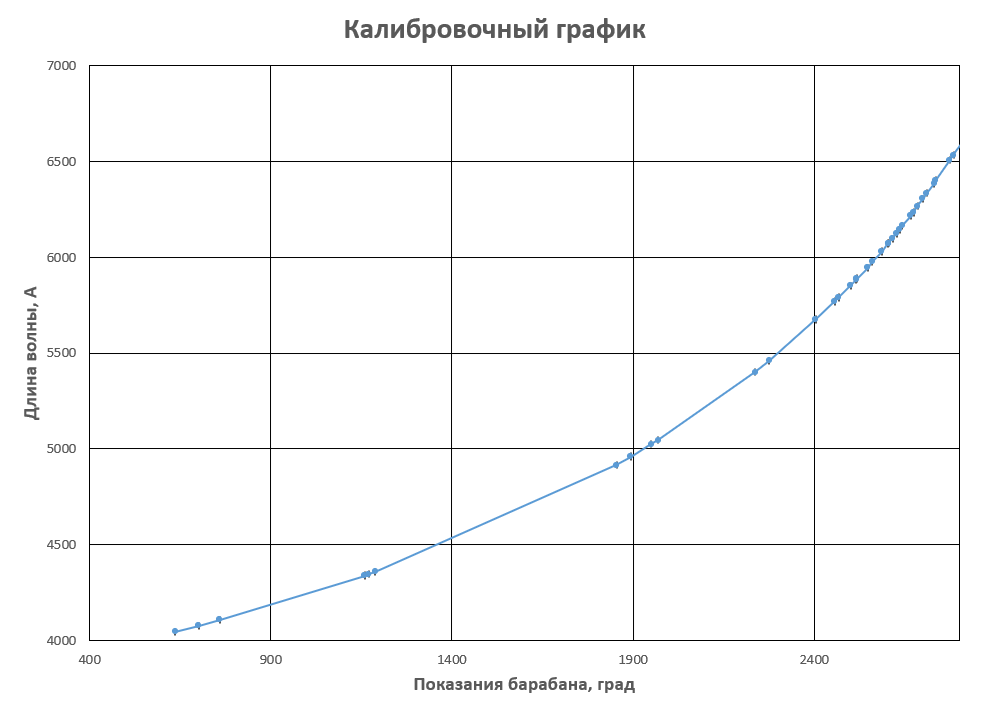
\includegraphics[scale=0.7]{grad.png}\newline
Рис.1. Градуировочный график
\end{center}



\subsection{Изучение спектра атома водорода}



Определим длины волн четырех линий серии Бальмера для $n = 2$ и вычислим значения 


		\begin{table}[h!]
		\caption{Определение линий спектра водорода}
		\begin{center}
			\begin{tabular}{|c|c|c|c|c|c|c|}
				\hline 
				Линия спектра &  барабан $^\circ $ & $ \lambda, \;\mathring{A} $ & $ m $ & R, cm^{-1} & $\sigma \lambda$, A & $\sigma R$, cm^{-1} \\ 
				\hline 
			$ H_\alpha $ & 2796 & 6567.4 & 3 & 109631.8 & 5.6 & 93.48 \\
		$ H_\beta $  & 1800 & 4861.4 &     4 & 109495.6 & 3.1 & 69.69 \\
			$ H_\gamma $ & 1160 & 4340.5 & 5 & 109723.1 & 1.8 & 44.75 \\
			$ H_\delta $ & 746 & 4101.7 &  6 & 109732.3 & 1.6 & 42.81 \\
				\hline 
			\end{tabular} 
		\end{center}
		\label{table_mn}
	\end{table}

\newpage

Вычислил значение постоянной Ридберга для каждых четырех линий серии Бальмера. Получаем:

$$R = 109645.7 \pm 33.01, cm^{-1}$$

$$\sigma_R = \frac{R}{\lambda} \sigma_\lambda$$

Табличное значение постоянной Ридберга: $R = 109677.6$, $cm^{-1}$. Вычисленное значение совпадает с табличным в пределах погрешности.






\subsection{Изучение молекулярного спектра йода.}

Запишем положения барабана для различных линий спектра йода (таблица 4).

		\begin{table}[h!]
		\caption{Определение линий спектра йода}
		\begin{center}
			\begin{tabular}{|c|c|c|c|c|c|c|c|c|c|c|c|c|}
				\hline 
			1 серия & 2754 & 2739 & 2724 & 2706 & 2689 & 2673 & 2653 & 2639 & 2621 & 2604 & 2587 & 2569 \\ \hline
		      
			2 серия & 2442 & 2424 & 2405 & 2398 & 2355 & 2339 & 2307 & 2291 & 2275 & 2245 & 2230 & 2217  \\
			2 серия & 2442 & 2424 & 2405 & 2398 & 2355 & 2339 & 2307 & 2291 & 2275 & 2245 & 2230 & 2217  \\
			2 серия & 2442 & 2424 & 2405 & 2398 & 2355 & 2339 & 2307 & 2291 & 2275 & 2245 & 2230 & 2217  \\
				\hline 
			\end{tabular} 
		\end{center}
		\label{table_mn}
	\end{table}

		\begin{table}[h!]

		\begin{center}
			\begin{tabular}{|c|c|c|c|c|c|c|c|c|c|c|c|c|}
				\hline 
			1 серия & 2552 & 2534 & 2514 & 2498 & 2479 & 2460 & 2442 & 2428 & 2409 & 2393 & 2377 & 2361 \\
		      
			2 серия & 2189 & 2176 & 2151 & 2139 & 2126 & 2114 & 2070 & 2060 & 2051 & 2033 & 2025 & 2018  \\
				\hline 
			\end{tabular} 
		\end{center}
		\label{table_mn}
	\end{table}
	
			\begin{table}[h!]

		\begin{center}
			\begin{tabular}{|c|c|c|c|c|c|c|c|c|c|c|c|c|}
				\hline 
			1 серия & 2346 & 2331 & 2314 \\
		      
			2 серия & 1990 & 1984 & 1978 \\
				\hline 
			\end{tabular} 
		\end{center}
		\label{table_mn}
	\end{table}
	
	

В таблицу 5 запишем длины трех линий: $h\nu(1,0)$ - красная,  $ h\nu(1,5) $ - желтая, $ h\nu(\text{гр}) $ - фиолетовая.

		\begin{table}[h!]
		\caption{Определение линий спектра йода}
		\begin{center}
			\begin{tabular}{|c|c|c|c|c|c|c|c|c|c|c|}
				\hline 
				Линия & Барабан & $ \lambda, A$ & $ \nu $, ТГц & $h\nu$, эВ & $\sigma \lambda$, A & $\sigma_\nu$, ТГц & $\sigma_{h\nu}$, эВ \\ 
				\hline 
			$ h\nu(1,0) $ & 2754 & 6451.74 & 464.991 & 1.925 & 5.84 & 0.421 & 0.002 \\
		    $ h\nu(1,5) $  & 2673 & 6232.02 & 481.385 & 1.993 & 8.01 & 0.619 & 0.003\\
			$ h\nu(\text{гр}) $ & 1978 & 5057.75 & 593.149 & 2.456 & 5.12 & 0.600 & 0.002\\
				\hline 
			\end{tabular} 
		\end{center}
		\label{table_mn}
	\end{table}


\newpage


Вычислим в электрон-вольтах энергию колебательного кванта возбужденного состояния молекулы йода:
\[\nu = c / \lambda\]
\[\sigma_{\nu} = \frac{c}{\lambda^2}\cdot \sigma_{\lambda}\]

\[h\nu_2 =\frac{h\nu_{1,5} - h\nu_{1, 0}}{5} = \frac{1.925-1.993}{5}=0.013\pm 0.004eV\]

Энергия электронного перехода $h\nu_{el}$:
\[ h\nu_{el} = h\nu_{1,0}+h\nu_1 = 1.993+0.027 = 2.020\pm0.003eV\]


Энергия диссоциации молекулы в основном состоянии $D_1$:
\[D_1 = h\nu_{gr} - E_A = 2.456-0.940=1.516\pm0.003eV\]


Энергия диссоциации молекулы в возбужденном состоянии $D_2$:
\[D_2 = h\nu_{gr} - h\nu_{el} = 2.456 - 2.020 = 0.436\pm0.006eV\]




Зная, что $h\nu_1 = 0.027$ эВ, $E = 0.94$ эВ, то $D_1 = 1.5425 \pm 0.004$ эВ, $D_2=0.69 \pm 0.008$ эВ.


\section{Вывод}

В работе исследовались сериальные закономерности в оптическом спектре водорода и спектр поглощения паров йода в видимой области.
	
	С помощью информации о спектральных линиях неона и ртути проградуирован спектрометр. Построен соответствующий график.
	
	Получены длины волн линий $H_{\alpha}$, $H_{\beta}$, $H_{\gamma}$ и $ H_\delta $ серии Бальмера, вычислена постоянная Ридберга. В рамках погрешности данные совпали с табличными.
	
	$$R = 109645.7 \pm 33.01, cm^{-1}$$
	
	Получены длины волн, соответствующие некоторым электронно-колебательным переходам из основного состояния в возбуждённое. Вычислены энергия колебательного кванта возбуждённого состояния молекулы, энергия электронного перехода, энергии диссоциации молекулы в основном и в возбуждённом состояниях.


    $$D_1 = (1.5425 \pm 0.004)  \text{ эВ},\text{  } D_2 = (0.69 \pm 0.008) \text{ эВ}$$ \\





\addcontentsline{toc}{section}{Список используемой литературы}


\begin{thebibliography}{}

\bibitem{Sulsky1994}
Лабораторный практикум по общей физике: Учеб. пособие для вузов. Т. 3. Квантовая физика / Игошин Ф.Ф., Самарский Ю.А., Ципенюк Ю.М.; Под ред. Ципенюка Ю.М. - М.:Физматкнига, 2005. 432 стр.



	
\end{thebibliography}

\end{document}
